\documentclass{osa-article}

%% Select the journal you're submitting to
%% oe, boe, ome, osac, osajournal
\journal{osajournal}
% Key:
% Express journals must have the correct journal selected:
% {oe} Optics Express
% {boe} Biomedical Optics Express
% {ome} Optical Material Express
% {osac} OSAC Continuum
% Other OSA journals may use:
% {osajournal} Applied Optics, Advances in Optics and Photonics, Journal of the Optical Society of America A/B, Optics Letters, Optica, Photonics Research

% Uncomment if submitting to Photonics Research.
% ONLY APPLICABLE FOR \journal{osajournal}
% \setprjcopyright

% Set the article type
\articletype{Research Article}
% Note that article type is not required for Express journals (OE, BOE, OME and OSAC)

% Talon's custom commands
\newcommand{\argmin}{\arg\!\min}
\newcommand{\me}{\mathrm{e}}
\providecommand{\e}[1]{\ensuremath{\times 10^{#1}}} 
\providecommand{\mb}[1]{\mathbf{#1}}
\providecommand{\mf}[1]{\mathfrak{#1}}
\providecommand{\mc}[1]{\mathcal{#1}}
\providecommand{\ro}{\mathbf{\mathbf{r}}_o}
\providecommand{\so}{\mathbf{\hat{s}}_o}
\providecommand{\rb}{\mathbf{r}_b}
\providecommand{\rbm}[1]{r_b^{\text{m}}}
\providecommand{\rd}{\mathbf{r}_d}
\providecommand{\rdf}{\mathpzc{r}_d}
\providecommand{\mh}[1]{\mathbf{\hat{#1}}}
\providecommand{\mbb}[1]{\mathbb{#1}}
\providecommand{\bs}[1]{\boldsymbol{#1}}
\providecommand{\bv}{\bs{\nu}}
\providecommand{\bsh}[1]{\hat{\boldsymbol{#1}}}
\providecommand{\nan}{\left(\frac{\text{NA}}{n_o}\right)}
\providecommand{\lmsum}{\sum_{l=0}^\infty\sum_{m=-l}^{l}}
\providecommand{\intr}[1]{\int_{\mbb{R}^{#1}}}
\providecommand{\ints}[1]{\int_{\mbb{S}^{#1}}}
\DeclareFontFamily{OT1}{pzc}{}
\DeclareFontShape{OT1}{pzc}{m}{it}{<-> s * [1.10] pzcmi7t}{}
\DeclareMathAlphabet{\mathpzc}{OT1}{pzc}{m}{it}
\usepackage{empheq}
\newcommand{\eqname}[1]{\tag*{#1}}
\newcommand*\widefbox[1]{\fbox{\hspace{1em}#1\hspace{1em}}}

\begin{document}

\title{Spatio-angular fluorescence microscopy I. Basic theory}

\author{Talon Chandler,\authormark{1,*} Author order TBD,\authormark{2,*} and Patrick La Rivi\`ere \authormark{1}}

\address{\authormark{1}University of Chicago, Department of Radiology, Chicago, Illinois 60637, USA\\
\authormark{2}Publications Department, The Optical Society, 2010 Massachusetts Avenue NW, Washington, DC 20036, USA\\
\authormark{3}Currently with the Department of Electronic Journals, The Optical Society, 2010 Massachusetts Avenue NW, Washington, DC 20036, USA}

\email{\authormark{*}talonchandler@talonchandler.com} %% email address is required

%\homepage{talonchandler@talonchandler.com} %% author's URL, if desired

%%%%%%%%%%%%%%%%%%% abstract %%%%%%%%%%%%%%%%
%% [use \begin{abstract*}...\end{abstract*} if exempt from copyright]

\begin{abstract*}
  We introduce the basic elements of a spatio-angular theory of fluorescence
  microscopy. We start by analyzing a paraxial single-view fluorescence
  microscope imaging an ensemble of in-focus fluorophores without using the
  monopole or scalar approximations. We define and calculate the spatio-angular
  transfer function (SATF) and show that fluorescence microscopes have an
  angular band limit. We demonstrate the value of the transfer function approach
  by efficiently simulating the imaging process with numerical phantoms.
  Notably, we show that information about the out-of-plane orientation of
  in-focus fluorophores is imaged in paraxial widefield fluorescence
  microscopes. We discuss the implications of our analysis for all quantitative
  fluorescence microscopy studies.
\end{abstract*}

\section{Introduction}
Fluorescence microscopes are widely used in biology [XXX], materials science
[XXX], and metrology [XXX] for measuring the distribution of fluorophores
throughout a sample. While an unprocessed fluorescence micrograph reports the
approximate distribution of fluorophores throughout a sample, all microscopes
are diffraction limited, so the image is a blurred version of the true
fluorophore distribution. Therefore, microscopists who are interested in optimal
measurements will perform a computational restoration to recover some of the
information lost during the imaging process.

Restoration techniques attempt to recover the true distribution of fluorophores
using the measured data and a model of the imaging process. A model of the
imaging process can be obtained theoretically (by mathematically modeling the
instrument under idealized conditions), experimentally (by measuring the
instrument's response to a known input), or by a combination of theory and
experiment (by measuring parameters of an instrument model). In all cases the
accuracy of the restored fluorophore distribution is limited by the accuracy of
the imaging model.

All theoretical imaging models of make simplifying approximations that limit the
accuracy of restorations, so it is important to verify that the approximations
introduce an acceptable level of error. This work investigates the errors
introduced by two common approximations in models of fluorescence
microscopes---the \textit{monopole approximation} and the \textit{scalar
  approximation}.

by ignoring the
dipole excitation and emission processes and to (2) treat light propagation
under the \textit{scalar approximation} by ignoring the polarization of light.
These approximations can limit the accuracy of restoration in all types of
fluorescence microscopes. The goal of this work is to analyze fluorescence
microscopes without these approximations and find the conditions under which
these approximations are justified.

This work lies at the intersection of three classes of fluorescence microscopy:
(1) single-molecule localization microscopy (SMLM), (2) spatial ensemble
fluorescence microscopy including widefield, confocal, and light-sheet
techniques, and (3) polarized fluorescence microscopy. We briefly review these
three classes and focus on their use of the monopole and scalar approximations.

The SMLM community has pioneered the use of rigorous electromagnetic models of
fluorescence microscopes \cite{backer2014, lieb2004} [Novotny]. When a single
molecule is fluorescing in the sample, the measured intensity pattern is
strongly dependent on the orientation of the emitting molecule. Backlund and Lew
\cite{backlund2014} have shown that ignoring the orientation of fluorophores can
bias position estimates. Therefore, the most accurate SMLM experiments must
jointly estimate the position and orientation of each molecule.

A major limitation of SMLM experiments is speed

Meanwhile, most fluorescence microscopists image ensembles of fluorophores and
restore their images without considering the role that the monopole and scalar
approximations play in the restoration process. A typical fluorescence
microscopist is only interested in the spatial distribution of fluorophores, so
they reason (possibly erroneously) that they can ignore the orientation of the
emitters.

A smaller community of microscopists is interested in measuring the orientation
of ensembles of fluorophores \cite{mehta2016} [Forkey, Goldman, Moerner].
These techniques typically use a combination of 
Current restoration techniques use a model of the dipole excitation and emission
process to restore the orientation of fluorophores using pixel-wise arithmetic,
but these techniques do not perform any spatial restoration so they are
sub-optimal. To our knowledge no work has been done to model the complete
spatio-angular response of fluorescence microscopes to ensembles of oriented
fluorophores.

In this work we model ensembles of in-focus dipole absorber/emitters using
electromagnetic optics and the paraxial approximation. In section 2 we model the
excitation and detection processes of dipoles, and we define the most important
quantity in this work---the spatio-angular transfer function (SATF). We
calculate the SATF and show that fluorescence microscopes have an angular band
limit. In section 3 we perform simulations and compare our model to traditional
scalar models. In section 4 we discuss the implications of our work for
fluorescence microscopy and lay out a path towards a complete spatio-angular
theory of fluorescence microscopy.

\section{Theory}
Consider a single dipole radiator at the origin with its dipole moment oriented
along a direction $\so$. The dipole emitter creates a time-harmonic electric
field at a position $\mb{r}$ far from the dipole proportional to
\begin{align}
  \mb{E}_{\text{ff}}(\mb{r}, \so) \propto \frac{\text{exp}[ik|\mb{r}|]}{|\mb{r}|}\, \mh{r}\times\so\times\mh{r}.\label{eq:dip}
\end{align}
A typical approach to deriving Equation \ref{eq:dip} is to (1) use Maxwell's
equations to derive the inhomogeneous electromagnetic wave equations then (2)
use potentials to solve the wave equations with a dipole source term, then (3)
drop the terms that decay faster than $1/|\mb{r}|$---see Jackson, Novotny, Teich
for clear expositions. Equation~\ref{eq:dip} succinctly shows that dipole
radiators emit spherical wavefronts of polarized light with amplitude
proportional to $\cos\theta$ where $\theta$ is the angle between the field point
$\mb{r}$ and the dipole axis $\so$.

Many models of fluorophores approximate the vector field on the left hand side
of Equation \ref{eq:dip} with a scalar field---the \textit{scalar
  approximation}---and drop the orientation dependence on the right hand
side---the \textit{monopole approximation}. The approximated field is given by
\begin{align}
  U_{\text{ff}}(\mb{r}) \propto \frac{\text{exp}[ik|\mb{r}|]}{|\mb{r}|}. \label{eq:mono}
\end{align}
Models that use Equation \ref{eq:mono} as a starting point do not account for
polarization or dipole orientation effects. In Section \ref{sec:monopole} we
will review the derivation of the monopole imaging model starting with Equation
\ref{eq:mono}. These results are widely known, but they serve as a review of the
concepts we will need for the dipole imaging case. In Section \ref{sec:dipole}
will derive a dipole imaging model starting with Equation \ref{eq:dip}. Finally,
in Section \ref{sec:trans} we will calculate the SATF for the dipole imaging
model.

\subsection{Monopole imaging model}\label{sec:monopole}
We briefly analyze a paraxial 4$f$ fluorescence imaging system using the
monopole and scalar approximations---a similar treatment can be found in
\cite{goodman1996}. We start by considering a field of in-focus monopoles that
have been excited by a spatially uniform beam. As the fluorophores relax, they
emit scalar waves in the form of Equation \ref{eq:mono}. The waves propagate
through the microscope and we measure the irradiance on a two dimensional
detector.

We can represent the object as a two-dimensional function $f(\ro)$ that we call
the \textit{monopole density}---the number of monopoles at position $\ro$ per
unit area. In the language of image science, we say that $f(\ro)$ is a member of
the set of square integrable functions on the plane $\mbb{L}_2(\mbb{R}^2)$. The
data we collect is the irradiance on a plane $g(\rd)$, so the data is a member
of the same set $\mbb{L}_2(\mbb{R}^2)$.

A reasonable starting point is to assume that the relationship between the
object and the data is \textit{linear}---this seems plausibly since a scaled sum
of monopoles will result in a scaled sum of the irradiance patterns created by
the individual monopoles. Therefore, we can write the irradiance as the integral
over a field of monopoles weighted by the detector response due to single
monopoles
\begin{empheq}[box=\widefbox]{gather}
g(\rd{}) = \int_{\mbb{R}^2}d\ro{}\, h(\rd{}, \ro{})f(\ro{}). \label{eq:fwdmono} \\ \text{Monopole imaging model} \nonumber 
\end{empheq}
where $h(\rd{}, \ro{})$ is the kernel of the integral transform. 


The first step is to calculate the field in the back focal plane of the
objective lens. We can model a paraxial thin lens as a quadratic phase element,
so it converts a spherical wave to a plane wave in the back focal plane with a
sharp cutoff at the exit pupil of the lens
\begin{align}
  U_{\text{bfp}}(\mb{r}_b) \propto \Pi\left(\frac{|\mb{r}_b|}{\alpha}\right) \equiv
  \begin{cases}
    1\quad \text{if}\quad |\mb{r}_b| < \alpha,\\
    0\quad \text{else}.
  \end{cases}
\end{align}
A central result of Fourier optics is that the fields one focal distance from
either side of a paraxial lens are related by a scaled two-dimensional Fourier
transform. If we place a detector in the focal plane of the tube lens then the
field on the detector is given by
\begin{align}
  U_{\text{det}}(\mb{r}_d) \propto \mc{F}_{\mbb{R}^2}\left\{U_{\text{bfp}}(\mb{r}_b)\right\} = \frac{J_1(k\alpha|\mb{r}_d|)}{k\alpha|\mb{r}_d|}.
\end{align}
Finally, the detector measures the irradiance instead of the field, so we take
the modulus squared of the field to find that the measurable image of a single
monopole radiator at the origin is the familiar Airy disk
\begin{align}
  h(\mb{r}_d, \ro = 0) \propto |U_{\text{det}}(\mb{r}_d)|^2 = \left[\frac{J_1(k\alpha|\mb{r}_d|)}{k\alpha|\mb{r}_d|}\right]^2.
\end{align}
Shifting the monopole in the transverse plane will introduce a linear phase
factor in the back focal plane which will manifest as a shift on the detector.
Therefore, our imaging system is shift invariant and we can rewrite the
irradiance on the detector due to a monopole at $\ro$ as
\begin{align}
  h(\rd, \ro) = h(\rd - \ro). \label{eq:shift}
\end{align}
For convenience we have used the same letter for both functions in Equation
\ref{eq:shift} even though they have a different number of variables. We will
continue to rewrite functions with fewer variables in the same way throughout
this paper. Also, Equation \ref{eq:shift} only applies directly to microscopes
with unit magnification, but a similar relationship can be found for magnifying
microscopes by making a change of variables---see Barrett section 7.2.7.

Rotating a monopole will leave its image unchanged. Therefore, our imaging
system is rotation invariant and we can simplify the kernel further with
\begin{align}
  h(\rd - \ro) = h(|\rd - \ro|). \label{eq:rotational}
\end{align}

In the language of image science, Equation \ref{eq:fwdmono} specifies an
integral transform relationship between objects that are members of the space of
square-integrable functions on the plane $\mbb{U} = \mbb{L}_2(\mbb{R}^2)$ and
data that lives in the same space $\mbb{V} = \mbb{L}_2(\mbb{R}^2)$. We can
rewrite Equation \ref{eq:fwdmono} more abstractly as
\begin{align}
  \mb{g} = \mc{H}\mb{f} \label{eq:abstract}
\end{align}
where $\mc{H}: \mbb{L}_2(\mbb{R}^2) \rightarrow \mbb{L}_2(\mbb{R}^2)$ is the
forward operator of the imaging system. We say that the shift invariance and
rotational invariance introduced in Equations \ref{eq:shift} and
\ref{eq:rotational} are \textit{symmetries of the forward operator}. Specifying
a linear operator that maps $\mbb{L}_2(\mbb{R}^2)$ to $\mbb{L}_2(\mbb{R}^2)$
always requires us to specify a kernel in the set $\mbb{L}_2(\mbb{R}^4)$, but we
can exploit the symmetries of the forward operator to specify the complete
kernel with a ``smaller'' function in the set $\mbb{L}_2(\mbb{R})$.

Just as a finite-dimensional linear operator can be represented by a matrix in a
specific basis, the infinite-dimensional linear operator in Equation
\ref{eq:abstract} can be represented by an integral transform in a specific
basis. Equation \ref{eq:fwdmono} is an integral transform representation of the
monopole imaging process in a \textit{spatial basis} with basis functions of the
form $\delta(\mb{r} - \ro)$, but this is not always the best choice. We can
exploit the shift-invariance of the forward operator by choosing basis functions
of the form $\text{exp}[i2\pi \mb{r}\cdot\bs{\nu}]$ and use the Fourier
transform to reexpress the monopole imaging model in a \textit{spatial-frequency
  basis} as
\begin{align}
  G(\bs{\nu}) = H(\bs{\nu})F(\bs{\nu})\label{eq:freq}
\end{align}
where $\bs{\nu}$ is a two-dimensional spatial frequency, $G(\bs{\nu})$ is the
spectrum of the irradiance, $F(\bs{\nu})$ is the spectrum of the monopole
density, and $H(\bs{\nu})$ is the two-dimensional optical transfer function.
Because the fast Fourier transform provides an efficient method to change
between the spatial and spatial-frequency bases, Equation \ref{eq:freq} provides
a computational advantage over Equation \ref{eq:fwdmono} because we only need to
multiply two functions in $\mbb{L}_2(\mbb{R}^2)$.

The optical transfer function above exploits shift invariance but does not
exploit rotational invariance. We can define a similar transfer function that
exploits both shift and rotational invariance by choosing the same Fourier basis
(see Barrett 7.2.9 for related discussion) and express the transfer function
as a member of the set $\mbb{L}_2(\mbb{R})$
\begin{align}
  G(\bs{\nu}) = H(|\bs{\nu}|)F(\bs{\nu}).\label{eq:freq2}
\end{align}
% Again, we have used the same letter symbol $H$ in Equations \ref{eq:freq} and
% \ref{eq:freq2} to denote a function with two real variables and one real
% variable, respectively.

\begin{figure}[h]
 \centering
   \centering
   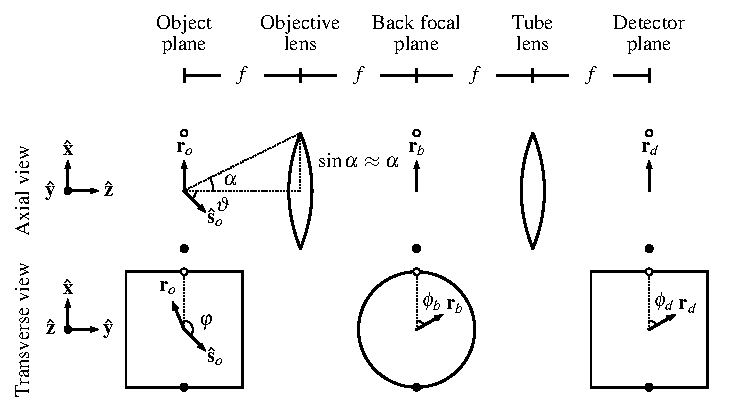
\includegraphics[scale=.9]{../figures/detection-coords/detection-coords.pdf}
   \caption{Detection geometry and coordinates.}
   \label{fig:mono}
 \end{figure}
\begin{figure}[h]
 \centering
   \centering
   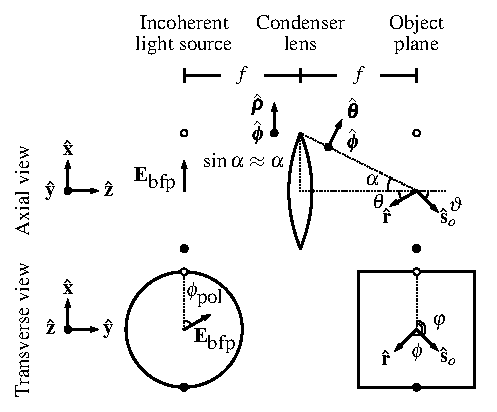
\includegraphics[scale=.9]{../figures/excitation-coords/excitation-coords.pdf}
   \caption{Illumination geometry and coordinates.}
   \label{fig:microscope}
 \end{figure}

\subsection{Dipole imaging model}\label{sec:dipole}
We seek to extend the monopole imaging model to dipoles. Comparing Equations
\ref{eq:dip} and \ref{eq:mono} shows that we will need to consider the
orientation of the dipole radiators. We also notice that both monopoles and
dipoles emit spherical wavefronts, so our argument for shift invariance in the
monopole imaging model holds for the dipole imaging model as well. Finally, it
is reasonable to assume that rotational invariance will be maintained under the
paraxial approximation. Therefore, we can plausibly extend the monopole imaging
model in Equation \ref{eq:fwdmono} to dipoles with
\begin{empheq}[box=\widefbox]{gather}
g(\rd{}) = \int_{\mbb{S}^2}d\so{}\int_{\mbb{R}^2}d\ro{}\, h(\rd{}, \ro{}, \so{})f(\ro, \so). \label{eq:fwddip}\\ \text{Dipole imaging model}\nonumber 
\end{empheq}
where $f(\ro, \so)$ is the \textit{spatio-angular density}---the number of
dipoles at position $\ro{}$ per unit area oriented along $\so{}$ per unit solid
angle---and $\mbb{S}^2$ is the unit sphere. Notice that the functional form of
our data is left unchanged $\mbb{V} = \mbb{L}_2(\mbb{R}^2)$ while we have
extended the set of possible objects to
$\mbb{U} = \mbb{L}_2(\mbb{R}^2\times\mbb{S}^2)$. Similar to the monopole case,
the most general linear operator mapping between these two spaces would require
a kernel in $\mbb{L}_2(\mbb{R}^4\times\mbb{S}^2)$, but we can exploit symmetries
and specify the complete kernel with a function in
$\mbb{L}_2(\mbb{R}\times\mbb{S}^2)$.

At this point we have only asserted the plausibility of Equation
\ref{eq:fwddip}---we still need to calculate the form of the kernel
$h(r, \so{})$. Our first step is to notice that the kernel can be separated into
the product of an excitation part and a detection part
\begin{align}
  h(r, \so) = h_{\text{exc}}(\so)\,h_{\text{det}}(r, \so). \label{eq:kernelsep}
\end{align}
In the next two subsections we will calculate the excitation and detection
kernels explicitly.

\subsubsection{Dipole excitation model}
When we developed the monopole imaging model we ignored the excitation process
because we excited the fluorophores with a spatially uniform excitation beam and
monopoles have no orientation dependence. For the dipole imaging model we must
account for the excitation process because the excitation process is not
angularly uniform (except for carefully calibrated TIRF systems).

In this section we will calculate the excitation kernel $h_{\text{exc}}(\so)$
for epi-illuminationn microscopes. We can interpret $h_{\text{exc}}(\so)$ as the
relative probability of exciting a molecule with dipole orientation $\so$. Our
approach is similar to previous work \cite{fourkas2001, chandler2017}, but here
we consider unpolarized and incoherent illumination and restrict ourselves to
the paraxial approximation.

We start by expressing the dipole moment $\so{}$ in spherical coordinates [see
Fig. 1(a)] as
\begin{align}
  \so{} &= \cos\varphi\sin\vartheta\mh{x} + \sin\varphi\sin\vartheta\mh{y} + \cos\vartheta\mh{z}. \label{eq:spherical}
\end{align}
We can rewrite Eq. \ref{eq:spherical} in terms of spherical harmonic functions
(see Appendix \ref{sec:sph}) as
\begin{align}
  \so{} &=\sqrt{\frac{3}{4\pi}}\left[y_1^1(\vartheta, \varphi)\,\mh{x} + y_1^{-1}(\vartheta, \varphi)\,\mh{y} + y_1^0(\vartheta, \varphi)\, \mh{z}\right]. \label{eq:sphharm}
\end{align}
We place the dipole in the focal plane of an aplanatic and
polarization-preserving objective lens with its optical axis aligned with the
$\mh{z}$ axis. Next, we place a spatially incoherent, spatially uniform,
unpolarized thermal light source (or its image) in the back aperture of the
objective lens to illuminate the focal plane. In this geometry each point in the
back focal plane generates a plane wave that illuminates the sample.

To model the unpolarized light source we will use polarized ray tracing [cite
Torok] to find the response for a single polarized ray, then integrate over the
rays and polarizations to find the complete response. First, we model the
electric field at every point on the back focal plane as
\begin{align}
   \mb{E}_{\text{bfp}}(\phi_{\text{pol}}) &\propto \cos\phi_{\text{pol}}\mh{x} + \sin\phi_{\text{pol}}\mh{y}, \label{eq:bfp0}
\end{align}
where $\phi_{\text{pol}}$ is the polarization orientation and \{$\mh{x}$,
$\mh{y}$\} are transverse Cartesian basis vectors. Note that Eq. \ref{eq:bfp0}
describes the incoherent electric fields at every point in the back focal
plane--- it does not describe a coherent plane wave. Immediately after the lens
the electric field is
\begin{align}
  \mb{E}_{\text{ff}}(\theta, \phi, \phi_{\text{pol}}) \propto \left\{[\mb{E}_\text{bfp}(\phi_{\text{pol}})\cdot\bsh{\phi}]\,\bsh{\phi} + [\mb{E}_\text{bfp}(\phi_{\text{pol}})\cdot\bsh{\rho}]\,\bsh{\theta}\right\}\sqrt{\cos\theta}, \label{eq:bfp2ff}
\end{align}
where \{$\theta$, $\phi$\} are spherical coordinates, \{$\bsh{\rho}$,
$\bsh{\phi}$\} are cylindrical basis vectors, and \{$\bsh{\theta}$,
$\bsh{\phi}$\} are spherical basis vectors defined in Figure 1(a) and related by
\begin{align}
  \bsh{\rho} &= \cos\phi\mh{x} + \sin\phi\mh{y},\label{eq:rho}\\
  \bsh{\phi} &= -\sin\phi\mh{x} + \cos\phi\mh{y},\label{eq:phi}\\
  \bsh{\theta} &= \cos\phi\cos\theta\mh{x} + \sin\phi\cos\theta\mh{y} - \sin\theta\mh{z}.\label{eq:theta}               
\end{align}
In Eq. \ref{eq:bfp2ff} the
$[\mb{E}_\text{bfp}(\phi_{\text{pol}})\cdot\bsh{\phi}]\,\bsh{\phi}$ term models
s-polarized fields, the
$[\mb{E}_\text{bfp}(\phi_{\text{pol}})\cdot\bsh{\rho}]\,\bsh{\theta}$ term
models the rotation of p-polarized fields, and the $\sqrt{\cos\theta}$ term
models the apodization of an aplanatic lens. After plugging Eqs. \ref{eq:bfp0}, \ref{eq:rho}, \ref{eq:phi}, and \ref{eq:theta} into Eq. \ref{eq:bfp2ff} and applying the
paraxial approximation, the electric field immediately after the lens is given
by
\begin{align}
  \mb{E}_{\text{ff}}^{(p)}(\theta, \phi, \phi_{\text{pol}}) \propto \cos\phi_{\text{pol}}\mh{x} + \sin\phi_{\text{pol}}\mh{y} - \theta\cos(\phi - \phi_{\text{pol}})\mh{z}.\label{eq:eff}
\end{align}
The probability that a dipole oriented along $\so{}$ is excited by a ray with
electric field $\mb{E}$ is given by $|\mb{E}\cdot\so{}|^2$. Evaluating this
expression for each ray would be cumbersome if we used Eqs. \ref{eq:spherical}
and \ref{eq:eff} because we would need to simplify a large number of
trigonometric functions. Instead, we use Eqs. \ref{eq:sphharm} and \ref{eq:eff}
and use the real Gaunt coefficients (see Appendix A) to evaluate the products of
spherical harmonics. We find that
% [theta**2*cos(phi - phip)**2/2 + 0.5*sin(phip)**2 + 0.5*cos(phip)**2, 0, 0, 0, sqrt(15)*sin(2*phip)/10, -sqrt(15)*theta*sin(phip)*cos(phi - phip)/5, sqrt(5)*theta**2*cos(phi - phip)**2/5 - sqrt(5)*sin(phip)**2/10 - sqrt(5)*cos(phip)**2/10, -sqrt(15)*theta*cos(phip)*cos(phi - phip)/5, -sqrt(15)*sin(phip)**2/10 + sqrt(15)*cos(phip)**2/10]
\begin{align}
  |\mb{E}_{\text{ff}}^{(p)}(\theta, \phi, \phi_{\text{pol}}) \cdot \so{}|^2 \propto\, &\left[1 + \theta^2\cos^2(\phi - \phi_{\text{pol}})\right]y_0^0(\so{}) + \frac{1}{\sqrt{5}}\left[ - 1 + 2\theta^2\cos^2(\phi - \phi_{\text{pol}})\right]y_2^{0}(\so{}) +\nonumber \\
                                   &\frac{\sqrt{15}}{10}\theta\sin\phi_{\text{pol}}\cos(\phi - \phi_{\text{pol}})y_2^{-1}(\so{}) + \frac{\sqrt{15}}{10}\theta\cos\phi_{\text{pol}}\cos(\phi - \phi_{\text{pol}})y_2^{1}(\so{}) -\nonumber \\  
                                   &\frac{\sqrt{15}}{20}\sin(2\phi_{\text{pol}})y_2^{-2}(\so{}) - \frac{\sqrt{15}}{20}\cos(2\phi_{\text{pol}})y_2^{2}(\so{}).\label{eq:integrand}
\end{align}
To find the complete excitation kernel we need to integrate Eq.
\ref{eq:integrand} over all polarization orientations and rays
\begin{align}
  h_{\text{exc}}(\so{}) \propto \int_0^{\alpha}\theta d\theta\int_0^{2\pi}d\phi\int_0^{2\pi}d\phi_{\text{pol}}\, |\mb{E}_{\text{ff}}^{(p)} \cdot \so{}|^2, \label{eq:integral}
\end{align}
where $\alpha$ is the maximum angle the illumination rays make with the optical
axis ($\alpha$ is equivalent to the numerical aperture in the paraxial
approximation).

After plugging Eq. \ref{eq:integrand} into Eq. \ref{eq:integral} and evaluating
the integrals, all but two terms disappear and the 
excitation kernel is given by
\begin{align}
  h_{\text{exc}}(\so{}) &\propto \left[1 + \frac{\alpha^2}{4}\right]y_0^0(\so{}) + \frac{1}{\sqrt{5}}\left[-1 + \frac{\alpha^2}{2}\right]y_2^0(\so{}). \label{eq:excitation}
\end{align}
We note that the excitation kernel depends on the orientation of the molecule,
but it does not depend on the position of the molecule in the focal plane. This
is a direct consequence of our illumination geometry---we have placed incoherent
light sources in the back focal plane of the objective so each point in the
focal plane within the field of view is illuminated equally.

Equation \ref{eq:excitation} only contains $m = 0$ spherical harmonics, so it
can be written as a function of $\vartheta$ only. After plugging in the
spherical harmonic functions and simplifying we see that 
\begin{align}
  h_{\text{exc}}(\vartheta) &\propto \sin^2\vartheta + \frac{1}{2}\alpha^2\cos^2\vartheta \label{eq:hexctheta}
\end{align}


Equation \ref{eq:excitation} shows the probability of excitation as a function
of dipole orientation and numerical aperture.
\begin{figure}[h]
 % \captionsetup{width=1.0\linewidth}
 \centering
   \centering
   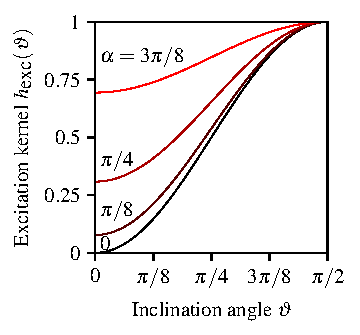
\includegraphics[scale=0.95]{../figures/excitation/excitation.pdf}
   \caption{Caption.}
   \label{fig:microscope}
 \end{figure}


\subsubsection{Dipole detection model}
In this section we will calculate the detection kernel of an epi-detection
microscope---the irradiance on the detector due to single molecule at a known
position with known orientation. Our approach mimics existing work
\cite{backer2014, nov2006, agrawal2012}, but we restrict ourselves to the
paraxial approximation.

We consider a single dipole emitter at the origin with a fixed dipole emission
moment oriented along $\so{}$. The electric field at a position $\mb{r}$ far
from the dipole is given by
\begin{align}
  \mb{E}_{\text{ff}}(\mb{r}, \so{}) \propto \frac{\text{exp}[ik|\mh{r}|]}{|\mh{r}|}\mh{r} \times \so{} \times \mh{r}. \label{eq:ff}
\end{align}
We place the dipole in the focal plane of the same 4$f$ imaging system we
considered in the monopole case---see Figure \ref{fig:monopole}. The dipole
emits spherical wavefronts so we can reuse our argument for shift invariance in
the monopole section and drop the phase dependence while keeping in mind that
$h_{\text{det}}(\rd, \ro, \so) = h_{\text{det}}(\rd - \ro, \so)$.
\begin{align}
  \mb{E}_{\text{ff}}(\mb{r}, \so{}) &\propto [\mb{I} - \mh{r}\mh{r}^{\dagger}]\so \\
\end{align}
\begin{align}
  \mh{r}(\theta,\phi) \approx \theta\cos\phi\mh{x} + \theta\sin\phi\mh{y} + \mh{z}
\end{align}
\begin{align}
  \mb{E}_{\text{ff}}(\theta, \phi, \so{}) &\propto 
  \begin{bmatrix}
    1 & 0 &-\theta \cos\phi\\
    0 & 1 &-\theta \sin\phi\\
    -\theta\cos\phi&-\theta \sin(\phi)&0    
  \end{bmatrix}\so
\end{align}
\begin{align}
  \mb{R}_{\text{obj}}(\theta, \phi) &=
  \begin{bmatrix}
    1 & 0 &-\theta \cos\phi\\
    0 & 1 &-\theta \sin\phi\\
    -\theta\cos\phi&-\theta \sin(\phi)&1    
  \end{bmatrix}
\end{align}

If we place the molecule in the focal plane of an aplanatic and
polarization-preserving objective lens with its optical axis aligned with the
$\mh{z}$ axis (or reuse the illumination objective), then the electric field in
the back focal plane of the lens is given by
\begin{align}
  \mb{E}_{\text{bfp}}(\theta, \phi, \so) &\propto \mb{R}_{\text{obj}}(\theta,\phi)\mb{E}_{\text{ff}}(\theta, \phi, \so)
\end{align}
Finally, we change from spherical coordinates to cylindrical coordinates by
substituting $(r_b, \phi_b)$ for $(\theta, \phi)$ and we get
\begin{align}
  \mb{E}_{\text{bfp}}(r_b, \phi_b, \so{}) \propto \left\{\left[s_x - s_zr_b\cos\phi_b\right]\mh{x} + \left[s_y - s_z r_b\sin\phi_b\right]\mh{y}\right\}\Pi\left(\frac{r_b}{\alpha}\right). \label{eq:bfp2}
\end{align}
\begin{align}
  \mb{E}_{\text{bfp}}(r_b, \phi_b, \so{}) \propto \left\{s_x\mh{x} + s_y\mh{y} + s_z r_b \mh{\bs{\rho}}\right\}\Pi\left(\frac{r_b}{\alpha}\right). \label{eq:bfp3}
\end{align}

We note that Eq. \ref{eq:bfp2} is identical to previously derived models
[Piestun, Backer] except here we have used the paraxial approximation and used
spherical harmonic functions.

Next we place a tube lens one focal length from the back focal plane and a
detector (see Figure XX)). Under the paraxial approximation we can find the
electric field in the detector plane by taking the Fourier transform of the
field in the back focal plane [Goodman]
\begin{align}
  \mb{E}_{\text{det}}^{(p)}(\rd{}, \so{}) &= \int_{\mbb{R}^2}d\rb{} \mb{E}_{\text{bfp}}^{(p)}(\rb{})\, \text{exp}\left[ik\,\rb{}\cdot\rd{}\right].\label{eq:det1}
\end{align}
To evaluate the integral we rewrite it in polar coordinates
\begin{align}
\mb{E}_{\text{det}}^{(p)}(\rd{}, \so{}) &= \int_{0}^{\alpha}r_bdr_b\int_0^{2\pi} d\phi_b\, \mb{E}_{\text{bfp}}^{(p)}(r_b, \phi_b)\, \text{exp}\left[ikr_b r_d\cos(\phi_b - \phi_d)\right],
\end{align}
substitute Eq. \ref{eq:bfp2}, and apply the following identities
\begin{align}
  \int_0^{2\pi}d\phi_b
  \left\{\substack{
    \sin(n\phi_b)\\
    \cos(n\phi_b)
  }\right\}
  \text{exp}\left[ikr_br_d\cos(\phi_b - \phi_d)\right] &= 2\pi i^n
  \left\{\substack{
    \sin(n\phi'_o)\\
    \cos(n\phi'_o)
  }\right\}J_n(k r_br_d),
  \end{align}
  \begin{align}
  \int_0^{\alpha} dr_b (r_b)^{n+1}J_{n}(kr_br_d) &= \alpha^{n+1}\left[\frac{J_{n+1}(k\alpha r_d)}{k r_d}\right],
  \end{align}
to find that 
\begin{align}
  \mb{E}_{\text{det}}^{(p)}(\rd{}, \so{}) \propto &\left[\frac{J_1(k\alpha r_d)}{k\alpha r_d}y_1^1(\so{}) - i\alpha \frac{J_2(k\alpha r_d)}{k\alpha r_d}\cos\phi_d y_1^0(\so{})\right]\mh{x}\, + \nonumber \\& \left[\frac{J_1(k\alpha r_d)}{k\alpha r_d}y_1^{-1}(\so{}) - i\alpha \frac{J_2(k\alpha r_d)}{k\alpha r_d}\sin\phi_d y_1^0(\so{})\right]\mh{y}.
\end{align}
We can find the irradiance on the detector by taking the modulus squared of the
electric field
\begin{align}
  h_{\text{det}}(\rd{}, \so{}) &\propto |\mb{E}_{\text{det}}^{(p)}(\rd{}, \so{})|^2.
\end{align}
We use the real Gaunt coefficients to find that
\begin{align}
h_{\text{det}}(\rd{}, \so{}) &\propto \left[a_1( r_d) + \frac{\alpha^2}{4} a_2( r_d)\right]y_0^0(\so{}) + \frac{1}{\sqrt{5}}\left[- a_1( r_d) + \frac{\alpha^2}{2} a_2( r_d)\right]y_2^0(\so{}), \label{eq:detection}
\end{align}
where we have defined
\begin{align}
  a_n(r_d) \equiv \frac{n}{\pi}\left[\frac{J_n(k\alpha r_d)}{k\alpha r_d}\right]^2. 
\end{align}
Similar to the excitation kernel, we can write the excitation kernel purely in terms of
the inclination angle
\begin{align}
  h_{\text{det}}(r_d, \vartheta) &\propto a_1(r_d)\sin^2\vartheta + \frac{1}{2}\alpha^2a_2(r_d)\cos^2(\vartheta). 
\end{align}

In our analysis we have only considered a dipole radiator at the origin, but we
can use the shift-invariance of 4$f$ imaging systems to model dipole radiators
at arbitrary positions in the focal plane. If we shift the dipole radiator to an
in-focus position $\ro{}$, then the irradiance pattern on the detector will be
given by $h_{\text{det}}(\rd{} - \ro{})$. We have also restricted our analysis
to an imaging system with unit magnification, but an imaging system with an
arbitrary magnification can be modeled as a system with unit magnification using
a change of variables (see \cite{barrett2004} section 7.2.7).

Finally, we note the similarities between Eqs. \ref{eq:excitation} and
\ref{eq:detection}. If we integrate the detection kernel over the detector and
use the identity $\int_{\mbb{R}^2}d\mb{r}\, a_n(r) = 1$ for $n \in \mbb{N}$,
then we find that the excitation and detection kernels are related by
\begin{align}
  h_{\text{exc}}(\so{}) = \int_{\mbb{R}^2}d\mb{r} h_{\text{det}}(\mb{r}, \so{}).
\end{align}

\begin{figure}[h]
 % \captionsetup{width=1.0\linewidth}
 \centering
   \centering
   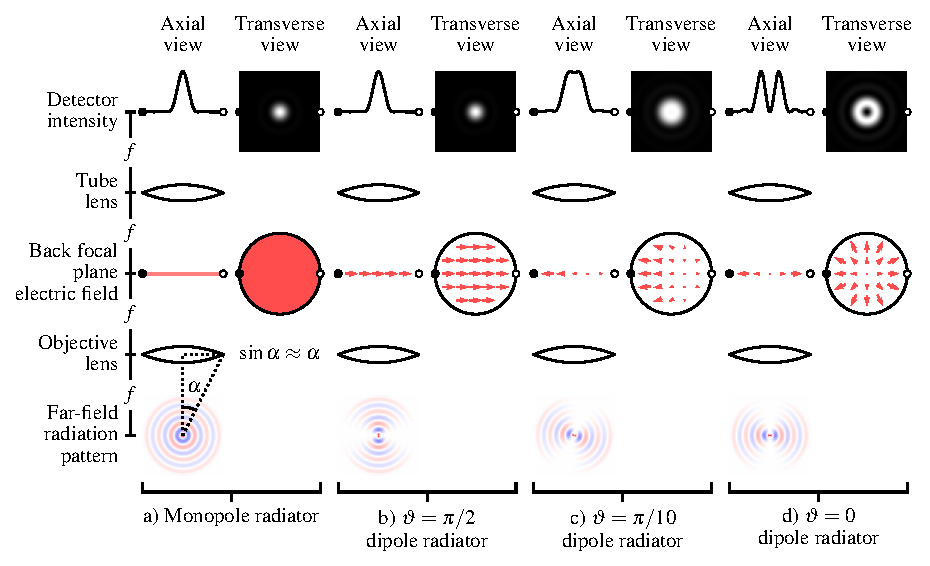
\includegraphics[scale=0.8]{../figures/microscope/microscope.pdf}
   \caption{Comparison of paraxial detection models for monopole radiators a)
     and dipole radiators b)--d). Monopole radiators fill the back focal plane
     with a uniform scalar field which gives rise to the familiar Airy disk on
     the detector. A transverse dipole radiator also creates an Airy disk---the
     back focal plane is filled with a uniform vector field. An axial dipole
     radiator creates a radial electric field pattern in the back focal plane
     which gives rise to a higher-order Airy disk. Back focal plane electric
     fields from transverse dipoles are purely even while fields from axial
     dipoles are purely odd which causes a relative $\pi/2$ phase shift for the
     fields on the detector. The back focal plane fields from an
     arbitrarily-oriented dipole can be decomposed into even and odd fields, so
     the final intensity pattern is always radially symmetric.}
   \label{fig:microscope}
 \end{figure}

\begin{figure}[h]
 % \captionsetup{width=1.0\linewidth}
 \centering
   \centering
   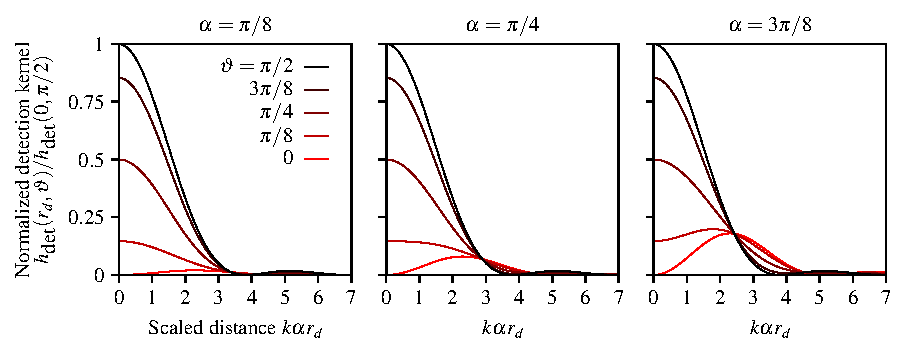
\includegraphics[scale=0.8]{../figures/detection/detection.pdf}
   \caption{Normalized detection kernel as a function of the scaled radial
     detection coordinate $k\alpha r_d$, the dipole inclination angle
     $\vartheta$, and the collection angle $\alpha$. For small collection angles
     (left) the detection kernel of axial dipoles
     (\textcolor{red}{\textbf{red}}) is small compared to transverse dipoles
     (\textbf{black}), but the relative contribution of axial dipoles increases
     with the collection angle (see \textcolor{red}{\textbf{red}} lines from left to right).}
   \label{fig:microscope}
 \end{figure}
 


 \subsection{Spatio-angular transfer function}\label{sec:trans}
 \begin{align}
g(\rd{}) = \int_{\mbb{S}^2}d\so{}\int_{\mbb{R}^2}d\ro{}\, h(|\rd{} -\ro{}|, \so{})f(\ro, \so).
 \end{align}

 \begin{align}
   g(\rd{}) = \mc{F}^{-1}_{\mbb{R}^2}\left\{\int_{\mbb{S}^2}d\so{}\, \mc{F}_{\mbb{R}^2}\left\{h(|\rd{} -\ro{}|, \so{})\right\}\mc{F}_{\mbb{R}^2}\left\{f(\ro, \so)\right\}\right\}.
 \end{align}
\begin{align}
  \ints{2}d\mh{s}{}\, f(\mh{s})g(\mh{s}) = \lmsum \mc{F}_{\mbb{S}^2}\left\{f(\mh{s})\right\}\mc{F}_{\mbb{S}^2}\left\{g(\mh{s})\right\}, \label{eq:plan}
\end{align}
where
\begin{align}
  \mc{F}_{\mbb{S}^2}\left\{f(\mh{s})\right\} \equiv \int_{\mbb{S}^2}f(\mh{s})y_l^m(\mh{s}).
\end{align}
Eq. \ref{eq:plan} is the generalized Plancharel theorem for spherical functions.
It is a special case of the fact that scalar products are invariant under
unitary transformations (see Barrett 3.78). Next, we plug Eq. \ref{eq:plan}
into Eq. \ref{eq:filter1} to get
\begin{align}
  g(\rd) = \mc{F}^{-1}_{\mbb{R}^2}\left\{\lmsum H_{l}^m(\bv, \mh{p}) \mc{F}_{\mbb{R}^2\times\mbb{S}^2}\left\{f(\ro, \so)\right\}\right\} \label{eq:filter}
\end{align}
where
\begin{align}
  H_{l}^m(\bv) \equiv \mc{F}_{\mbb{R}^2\times\mbb{S}^2}\left\{h(|\rd - \ro|, \so)\right\} &\equiv \intr{3}d\ro\, \me^{i2\pi\ro\cdot\bv}\ints{2}d\so\, y_l^m(\so) h(\ro, \so).\label{eq:transfer}
\end{align}
Eq. \ref{eq:filter} is the main result of this section. Right now it is not
obvious that Eq. \ref{eq:filter} is any more efficient than Eq.
\ref{eq:filter1}, but when we calculate the transfer function we will see that
the sum over spherical harmonics contains a small number of terms.


 
As written Eq. \ref{eq:fwd} is an extremely expensive integral to compute---to
find the irradiance at a single point on the detector we need to evaluate the
spatio-angular density and the kernel at every point in
$\mbb{S}^2\times \mbb{R}^2$. To simplify the integral, we expand the object and
the kernel onto complex exponentials and spherical harmonics using
\begin{align}
  F_l^m(\bs{\nu}) &\equiv \int_{\mbb{S}^2}d\so{}y_l^m(\so{})\int_{\mbb{R}^2}d\ro{}\,\text{exp}\left[i2\pi \ro{}\cdot\bs{\nu}\right]f(\ro{}, \so{}),\\
  H_l^m(\bs{\nu}) &\equiv \int_{\mbb{S}^2}d\so{}y_l^m(\so{})\int_{\mbb{R}^2}d\ro{}\,\text{exp}\left[i2\pi \ro{}\cdot\bs{\nu}\right]h(\ro{}, \so{}).
\end{align}
We also expand the detector irradiance onto spatial harmonics using the Fourier
transform
\begin{align}
  G(\bs{\nu}) \equiv \int_{\mbb{R}^2}d\rd{}\,\text{exp}\left[i2\pi \rd{}\cdot\bs{\nu}\right]g(\rd{}).
\end{align}
Given these definitions, we can rewrite Eq. \ref{eq:fwd} in the frequency domain as 
\begin{align}
G(\bs{\nu}) = \sum_{l=0}^{\infty}\sum_{m=-l}^{l}H_l^m(\bs{\nu})F_l^m(\bs{\nu}). 
\end{align}

In Appendix A we calculate the spatio-angular transfer function as
\begin{align}
  H_l^m(\bs{\nu}) = \frac{1}{C}\Bigg\{&\left[\left(1 + \frac{\alpha^2}{8}\right)A_1(\nu) + \left(\frac{\alpha^2}{8} + \frac{3\alpha^4}{32}\right)A_2(\nu)\right]\delta_{l0}\delta_{m0}+\nonumber\\&\frac{2\sqrt{5}}{7}\left[\left(-1 + \frac{\alpha^2}{16}\right)A_1(\nu) + \left(\frac{\alpha^2}{16} + \frac{3\alpha^4}{16}\right)A_2(\nu)\right]\delta_{l2}\delta_{m0}\nonumber\\&\frac{1}{7}\left[\left(1 - \frac{\alpha^2}{2}\right)A_1(\nu) + \left(-\frac{\alpha^2}{2} + \frac{\alpha^4}{4}\right)A_2(\nu)\right]\delta_{l4}\delta_{m0}\Bigg\}, 
\end{align}
where
\begin{align}
  A_1(\nu) &= \frac{2}{\pi}\left\{\cos^{-1}\left(\frac{\nu}{2\nu_o}\right) - \frac{\nu}{2\nu_o}\sqrt{1 - \left(\frac{\nu}{2\nu_o}\right)^2}\right\}\Pi\left(\frac{\nu}{2\nu_o}\right), \\
  A_2(\nu) &= \frac{2}{\pi}\Bigg\{\cos^{-1}\left(\frac{\nu}{2\nu_o}\right) - \left[3 - 2\left(\frac{\nu}{2\nu_o}\right)^2\right]\frac{\nu}{2\nu_o}\sqrt{1 - \left(\frac{\nu}{2\nu_o}\right)^2}\Bigg\}\Pi\left(\frac{\nu}{2\nu_o}\right), 
\end{align}
and $C = 1 + \frac{\alpha^2}{4} + \frac{3\alpha^4}{32}$ is a normalization
constant.

\section{Results}

\section{Discussion and conclusion}
Do microscopes transmit more information than Abbe thought?

Using an experimentally determined model is an effective way to find an accurate
model without understanding all of the physical details of the imaging system,
but these approaches require a known input that can completely characterize the
imaging system. Sub-diffraction beads are commonly used as a known input for
measuring the response of a microscope, but we argue that sub-diffraction beads
are not enough to completely characterize the response of a microscope to all
fluorescent samples. Beads can only characterize the response of the microscope
to an angularly uniform distribution of fluorophores, and we will show that all
microscopes have an orientation-dependent response. A complete characterization
requires a test sample with at least three known orientation distributions.

Can experimentally measured psfs account for this?

\bibliography{paper}
\appendix
\section{Spherical harmonics}\label{sec:sph}
The spherical harmonics are a basis for representing functions on the sphere. In
this appendix we will define the basis and review several important properties
of this set of functions. 

The complex-valued spherical harmonics are given by
\begin{align}
Y_l^m(\vartheta, \varphi) = \sqrt{\frac{(2l+1)(l-m)!}{4\pi(l+m)!}}\exp(i m \varphi)P_l^m\left(\cos\theta\right)
\end{align}
where $P_l^m(\cos\theta)$ are the associated Legendre polynomials that include
the Condon-Shortley phase. In this work we only use the spherical harmonics to
represent real-valued functions so we use the real spherical harmonics given by
\begin{align}
  y_l^m(\vartheta, \varphi)
  \begin{cases}
    \frac{Y_l^m(\vartheta, \varphi) + (-1)^m Y_l^{-m}(\vartheta, \varphi)}{\sqrt{2}} &\quad m > 0, \\
    Y_l^m(\vartheta, \varphi) &\quad m = 0, \\
    \frac{Y_l^m(\vartheta, \varphi) - (-1)^m Y_l^{-m}(\vartheta, \varphi)}{i \sqrt{2}} &\quad m < 0.\\
        \end{cases}
\end{align}

The $l=0, 1, 2$ spherical harmonics are given by
\begin{align}
  y_0^0(\vartheta, \varphi) &= \sqrt{\frac{1}{4\pi}}, \nonumber \\ 
  y_1^{-1}(\vartheta, \varphi) &= \sqrt{\frac{3}{4\pi}}\sin\varphi\sin\vartheta, \nonumber\\
  y_1^0(\vartheta, \varphi) &= \sqrt{\frac{3}{4\pi}}\cos\vartheta, \nonumber \\
  y_1^1(\vartheta, \varphi) &= \sqrt{\frac{3}{4\pi}}\cos\varphi\sin\vartheta, \nonumber \\
  y_2^{-2}(\vartheta, \varphi) &= \sqrt{\frac{15}{4\pi}}\sin\varphi\cos\varphi\sin^2\vartheta, \nonumber\\
  y_2^{-1}(\vartheta, \varphi) &= \sqrt{\frac{15}{4\pi}}\sin\varphi\sin\vartheta\cos\vartheta,\nonumber \\
  y_2^0(\vartheta, \varphi) &= \sqrt{\frac{5}{16\pi}}(3\cos^2\vartheta - 1), \nonumber \\ 
  y_2^{1}(\vartheta, \varphi) &= \sqrt{\frac{15}{4\pi}}\cos\varphi\sin\vartheta\cos\vartheta, \nonumber \\
  y_2^{2}(\vartheta, \varphi) &= \sqrt{\frac{15}{16\pi}}(\cos^2\varphi - \sin^2\varphi)\sin^2\vartheta. \label{eq:harmonics}
\end{align}

Real Gaunt coefficients

\section{Evaluating the spatio-angular transfer function}
In this appendix we will evaluate 
\begin{align}
    H_l^m(\bs{\nu}) &\propto \int_{\mbb{S}^2}d\so{}y_l^m(\so{})\int_{\mbb{R}^2}d\ro{}\,\text{exp}\left[i2\pi \ro{}\cdot\bs{\nu}\right]h(\ro{}, \so{}),\label{eq:whole}
\end{align}
where
\begin{align}
  h(\rd{} - \ro{}, \so{}) &\propto h_{\text{exc}}(\so{})h_{\text{det}}(\rd{} - \ro{}, \so{}),\label{eq:split}\\ 
  h_{\text{exc}}(\so{}) &\propto \left[1 + \frac{\alpha^2}{4}\right]y_0^0(\so{}) + \frac{1}{\sqrt{5}}\left[-1 + \frac{\alpha^2}{2}\right]y_2^0(\so{}),\\  
  h_{\text{det}}(\rd{}, \so{}) &\propto \left[a_1( r_d) + \frac{\alpha^2}{4} a_2( r_d)\right]y_0^0(\so{}) + \frac{1}{\sqrt{5}}\left[- a_1( r_d) + \frac{\alpha^2}{2} a_2( r_d)\right]y_2^0(\so{}),
\end{align}
and
\begin{align}
    a_n(r_d) \equiv \frac{n}{\pi}\left[\frac{J_n(k\alpha r_d)}{k\alpha r_d}\right]^2. 
\end{align}
First we plug Eq. \ref{eq:split} into Eq. \ref{eq:whole} and move the excitation
kernel out of the spatial integral
\begin{align}
    H_l^m(\bs{\nu}) &\propto \int_{\mbb{S}^2}d\so{}y_l^m(\so{})h_{\text{exc}}(\so{})\int_{\mbb{R}^2}d\ro{}\,\text{exp}\left[i2\pi \ro{}\cdot\bs{\nu}\right]h_{\text{det}}(\rd{}, \so{}). \label{eq:satf}
\end{align}
The spatial integral requires us to evaluate the two-dimensional Fourier
transform of $a_1(r_o)$ and $a_2(r_o)$. We will define
\begin{align}
  A_n(\nu) \equiv \mathcal{F}_2\{a_n(r_o)\} =  \int_{\mbb{R}^2}d\ro{}\,\text{exp}\left[i2\pi \ro{}\cdot\bs{\nu}\right] a_n(r_d), \label{eq:ftA}
\end{align}
and evaluate $A_1(\nu)$ and $A_2(\nu)$ later. After substituting \ref{eq:ftA}
into Eq. \ref{eq:satf} we find 
\begin{align}
  H_l^m(\bs{\nu}) \propto \int_{\mbb{S}^2}d\so{}y_l^m(\so{})&\left\{\left[1 + \frac{\alpha^2}{4}\right]y_0^0(\so{}) + \frac{1}{\sqrt{5}}\left[-1 + \frac{\alpha^2}{2}\right]y_2^0(\so{})\right\} + \nonumber\\&\left\{\left[A_1(\nu) + \frac{\alpha^2}{4} A_2(\nu)\right]y_0^0(\so{}) + \frac{1}{\sqrt{5}}\left[- A_1(\nu) + \frac{\alpha^2}{2} A_2(\nu)\right]y_2^0(\so{})\right\}. 
\end{align}
After expanding the products of spherical harmonics
\begin{align}
  H_l^m(\bs{\nu}) \propto \int_{\mbb{S}^2}d\so{}y_l^m(\so{})&\Bigg\{\left[\frac{3}{5}A_1(\nu) + \frac{3\alpha^2}{40}[A_1(\nu) + A_2(\nu)] + \frac{9\alpha^4}{160}A_2(\nu)\right]y_0^0(\so{})+\nonumber\\&\frac{3\sqrt{5}}{280}\left[-16A_1(\nu) + \alpha^2[A_1(\nu) + A_2(\nu)] + 3\alpha^4 A_2(\nu)\right]y_2^0(\so{})\nonumber\\&\frac{3}{35}\left[\left(1 - \frac{\alpha^2}{2}\right)A_1(\nu) + \left(-\frac{\alpha^2}{2} + \frac{\alpha^4}{4}\right)A_2(\nu)\right]y_4^0(\so{})\Bigg\},\\
  H_l^m(\bs{\nu}) \propto \int_{\mbb{S}^2}d\so{}y_l^m(\so{})&\Bigg\{\left[\left(1 + \frac{\alpha^2}{8}\right)A_1(\nu) + \left(\frac{\alpha^2}{8} + \frac{3\alpha^4}{32}\right)A_2(\nu)\right]y_0^0(\so{}) + \nonumber\\&\frac{\sqrt{5}}{56}\left[(-16 + \alpha^2)A_1(\nu) + (\alpha^2 + 3\alpha^4)A_2(\nu)\right]y_2^0(\so{})\nonumber\\&\frac{1}{7}\left[\left(1 - \frac{\alpha^2}{2}\right)A_1(\nu) + \left(-\frac{\alpha^2}{2} + \frac{\alpha^4}{4}\right)A_2(\nu)\right]y_4^0(\so{})\Bigg\}.
\end{align}
Next, we use the orthogonality of spherical harmonics to evaluate the angular integral
\begin{align}
  H_l^m(\bs{\nu}) = \frac{1}{C}\Bigg\{&\left[\left(1 + \frac{\alpha^2}{8}\right)A_1(\nu) + \left(\frac{\alpha^2}{8} + \frac{3\alpha^4}{32}\right)A_2(\nu)\right]\delta_{l0}\delta_{m0}+\nonumber\\&\frac{2\sqrt{5}}{7}\left[\left(-1 + \frac{\alpha^2}{16}\right)A_1(\nu) + \left(\frac{\alpha^2}{16} + \frac{3\alpha^4}{16}\right)A_2(\nu)\right]\delta_{l2}\delta_{m0}\nonumber\\&\frac{1}{7}\left[\left(1 - \frac{\alpha^2}{2}\right)A_1(\nu) + \left(-\frac{\alpha^2}{2} + \frac{\alpha^4}{4}\right)A_2(\nu)\right]\delta_{l4}\delta_{m0}\Bigg\}, 
\end{align}
where $C = 1 + \frac{\alpha^2}{4} + \frac{3\alpha^4}{32}$ is a normalization
constant.

Our final task is to calculate $A_1(\nu)$ and $A_2(\nu)$. $A_1(\nu)$ is a
well-known result \cite{goodman1996, mertz2009}, but we review the calculation
to establish the tools we'll need to evaluate $A_2(\nu)$. We start by using the
autocorrelation (Wiener-Khinchin) theorem to rewrite the Fourier transform as
\begin{align}
  A_1(\nu) = \frac{1}{\pi}\mathcal{F}_2\left\{\left[\frac{J_1(2\pi\nu_o r_o)}{2\pi\nu_o r_o}\right]^2\right\} = \frac{1}{\pi}\left[\mathcal{F}_2\left\{\frac{J_1(2\pi\nu_o r_o)}{2\pi\nu_o r_o}\right\} \star_2 \mathcal{F}_2\left\{\frac{J_1(2\pi\nu_o r_o)}{2\pi\nu_o r_o}\right\}\right] \label{eq:auto}
\end{align}
where $\star_2$ denotes a two-dimensional autocorrelation. Next, we recognize
that the Fourier transforms on the right hand side of Eq. \ref{eq:auto} are
rotationally symmetric so they can be rewritten as zero-order Hankel transforms
\begin{align}
  A_1(\nu) = \frac{1}{\pi}\left[\mathcal{H}_0\left\{\frac{J_1(2\pi\nu_o r_o)}{2\pi\nu_o r_o}\right\} \star_2 \mathcal{H}_0\left\{\frac{J_1(2\pi\nu_o r_o)}{2\pi\nu_o r_o}\right\}\right] \label{eq:autoz}
\end{align}
We can apply the Hankel transform identity \cite{poul1998}
\begin{align}
  \mathcal{H}_{n-1}\left\{\frac{J_n(2\pi\nu_o r_o)}{2\pi\nu_o r_o}\right\} = \frac{\nu^{n-1}}{\nu_o^{n}}\Pi\left(\frac{\nu}{\nu_o}\right),\label{eq:identity}
\end{align}
to find that 
\begin{align}
  A_1(\nu) = \frac{1}{\pi\nu_o^{2}}\left[\Pi\left(\frac{\nu}{\nu_o}\right) \star_2 \Pi\left(\frac{\nu}{\nu_o}\right)\right] \label{eq:auto3}. 
\end{align}
We can use the geometric construction in Figure \ref{fig:geometry} to express the
autocorrelation in terms of an integral over a region of overlap between
two circles given by
\begin{align}
  A_1(\nu) &= \frac{4}{\pi\nu_o^{2}}\left[\int_0^{\nu_o}\tau d\tau\int_0^{\cos^{-1}\left(\frac{\nu}{2\nu_o}\right)}d\phi_{\tau} - \int_{0}^{\nu/2}d\tau_x\int_0^{\tau_x\frac{2\nu_o}{\nu}\sqrt{1 - \left(\frac{\nu}{2\nu_o}\right)^2}}d\tau_y\right]\Pi\left(\frac{\nu}{2\nu_o}\right),\\
  A_1(\nu) &= \frac{4}{\pi\nu_o^{2}}\left[\int_0^{\nu_o}\tau d\tau\cos^{-1}\left(\frac{\nu}{2\nu_o}\right) - \int_{0}^{\nu/2}d\tau_x\tau_x\frac{2\nu_o}{\nu}\sqrt{1 - \left(\frac{\nu}{2\nu_o}\right)^2}\right]\Pi\left(\frac{\nu}{2\nu_o}\right),\\
  A_1(\nu) &= \frac{2}{\pi}\left\{\cos^{-1}\left(\frac{\nu}{2\nu_o}\right) - \frac{\nu}{2\nu_o}\sqrt{1 - \left(\frac{\nu}{2\nu_o}\right)^2}\right\}\Pi\left(\frac{\nu}{2\nu_o}\right).
\end{align}
\begin{figure}[h]
 % \captionsetup{width=1.0\linewidth}
 \centering
   \centering
   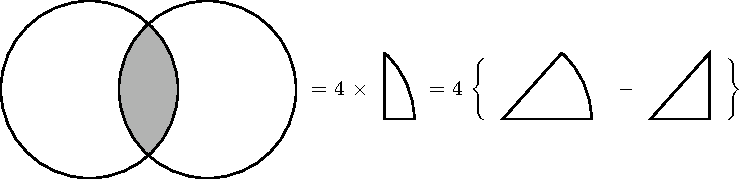
\includegraphics[width = 0.8\textwidth]{../figures/autocorrelation/autocorrelation.pdf}
   \caption{Geometric construction for evaluating the autocorrelations. We need
     to integrate over the overlapping region of two circles with radius $\nu_o$
     and distance $\nu$ between their centers. The region is given by four times
     the difference in area between a sector of angle
     $\arccos\left(\frac{\nu}{2\nu_o}\right)$ and a triangle with base $\nu/2$
     and hypotenuse $\nu_o$.}
   \label{fig:geometry}
 \end{figure}

 To evaluate $A_2(\nu)$ we could follow the same steps, but we will reach a dead
 end because there is no Hankel transform identity for
 $\mathcal{H}_{n-1}\left\{\frac{J_{n+1}(2\pi\nu_o r_o)}{2\pi\nu_o r_o}\right\}$.
 Instead, we rewrite $A_2(\nu)$ as
\begin{align}
  A_2(\nu) = \frac{2}{\pi}\mathcal{F}_2\left\{\left[\frac{J_2(2\pi\nu_o r_o)}{2\pi\nu_o r_o}\right]^2\right\} = \frac{2}{\pi}\left[\mathcal{F}_2\left\{\left[\frac{J_2(2\pi\nu_o r_o)}{2\pi\nu_o r_o}\cos\phi_{\nu}\right]^2\right\} + \mathcal{F}_2\left\{\left[\frac{J_2(2\pi\nu_o r_o)}{2\pi\nu_o r_o}\sin\phi_{\nu}\right]^2\right\}\right].
\end{align}
Applying the autocorrelation theorem gives
\begin{align}
  A_2(\nu) = \frac{2}{\pi}\Bigg[&\mathcal{F}_2\left\{\frac{J_2(2\pi\nu_o r_o)}{2\pi\nu_o r_o}\cos\phi_{\nu}\right\} \star_2 \mathcal{F}_2\left\{\frac{J_2(2\pi\nu_o r_o)}{2\pi\nu_o r_o}\cos\phi_{\nu}\right\} + \nonumber\\ &\mathcal{F}_2\left\{\frac{J_2(2\pi\nu_o r_o)}{2\pi\nu_o r_o}\sin\phi_{\nu}\right\} \star_2 \mathcal{F}_2\left\{\frac{J_2(2\pi\nu_o r_o)}{2\pi\nu_o r_o}\sin\phi_{\nu}\right\}\Bigg].
\end{align}
After converting the Fourier transforms to Hankel transforms with the identities
\begin{align}
  \mathcal{F}_2\left\{f(r)\cos(\phi)\right\} &= -i\cos\phi_{\nu}\mathcal{H}_1\left\{f(r)\right\},\\
  \mathcal{F}_2\left\{f(r)\sin(\phi)\right\} &= -i\sin\phi_{\nu}\mathcal{H}_1\left\{f(r)\right\},
\end{align}
and evaluating the Hankel transforms with Eq. \ref{eq:identity}, we find that
\begin{align}
  A_2(\nu) = -\frac{2}{\pi\nu_o^4}\left\{\left[\nu_x\Pi\left(\frac{\nu}{\nu_o}\right) \star_2 \nu_x\Pi\left(\frac{\nu}{\nu_o}\right)\right] + \left[\nu_y\Pi\left(\frac{\nu}{\nu_o}\right) \star_2 \nu_y\Pi\left(\frac{\nu}{\nu_o}\right)\right]\right\}. \label{eq:long}
\end{align}
Eq. \ref{eq:long} contains two autocorrelations that require us to find the
weighted overlap of two circles. Neither of these autocorrelations are
rotationally symmetric, but their sum must be rotationally symmetric. With this
symmetry in mind, we recognize that the first autocorrelation is largest for
shifts along the $x$ direction and smallest for shifts along the $y$ direction
with a smooth $\cos^2\phi_{\nu}$ weighting between the two extremes. The same is
true for the second autocorrelations except the $x$ and $y$ axes are exchanged
and there is a $\sin^2\phi_{\nu}$ weighting between the two extremes. Therefore,
we can rewrite Eq. \ref{eq:long} as
\begin{align}
  A_2(\nu) = -\frac{2}{\pi\nu_o^4}\Bigg\{&\left[\nu_x\Pi\left(\frac{\nu}{\nu_o}\right) \star_2^x \nu_x\Pi\left(\frac{\nu}{\nu_o}\right)\right]\cos^2\phi_\nu + \left[\nu_x\Pi\left(\frac{\nu}{\nu_o}\right) \star_2^y \nu_x\Pi\left(\frac{\nu}{\nu_o}\right)\right]\sin^2\phi_\nu + \nonumber\\ &\left[\nu_y\Pi\left(\frac{\nu}{\nu_o}\right) \star_2^x \nu_y\Pi\left(\frac{\nu}{\nu_o}\right)\right]\cos^2\phi_\nu + \left[\nu_y\Pi\left(\frac{\nu}{\nu_o}\right) \star_2^y \nu_y\Pi\left(\frac{\nu}{\nu_o}\right)\right]\sin^2\phi_\nu\Bigg\}. \label{eq:long3}
\end{align}
where $\star_2^x$ denotes a two-dimensional autocorrelation for shifts along
the $x$ direction. We can use the following pair of identities
\begin{align}
  \nu_x\Pi\left(\frac{\nu}{\nu_o}\right) \star_2^x \nu_x\Pi\left(\frac{\nu}{\nu_o}\right) = \nu_y\Pi\left(\frac{\nu}{\nu_o}\right) \star_2^y \nu_y\Pi\left(\frac{\nu}{\nu_o}\right),\\
  \nu_x\Pi\left(\frac{\nu}{\nu_o}\right) \star_2^y \nu_x\Pi\left(\frac{\nu}{\nu_o}\right) = \nu_y\Pi\left(\frac{\nu}{\nu_o}\right) \star_2^x \nu_y\Pi\left(\frac{\nu}{\nu_o}\right),
\end{align}
to simplify Eq. \ref{eq:long3} to
\begin{align}
  A_2(\nu) = -\frac{2}{\pi\nu_o^4}\Bigg\{&\left[\nu_x\Pi\left(\frac{\nu}{\nu_o}\right) \star_2^x \nu_x\Pi\left(\frac{\nu}{\nu_o}\right)\right] + \left[\nu_x\Pi\left(\frac{\nu}{\nu_o}\right) \star_2^y \nu_x\Pi\left(\frac{\nu}{\nu_o}\right)\right]\Bigg\}. \label{eq:long4}
\end{align}
First we evaluate the autocorrelation for shifts along the $x$ axis
\begin{align}
  &= -\frac{2}{\pi\nu_o^4}\left[\nu_x\Pi\left(\frac{\nu}{\nu_o}\right) \star_2^x \nu_x\Pi\left(\frac{\nu}{\nu_o}\right)\right]\\
  &= -\frac{8}{\pi\nu_o^4}\Bigg[\int_0^{\nu_o}\tau d\tau\int_0^{\cos^{-1}\left(\frac{\nu}{2\nu_o}\right)}d\phi_{\tau}(-\tau^2\cos^2\phi_{\tau} + \nu\tau\cos\phi_{\tau})\\ &\hspace{5em}- \int_{0}^{\nu/2}d\tau_x\int_0^{\tau_x\frac{2\nu_o}{\nu}\sqrt{1 - \left(\frac{\nu}{2\nu_o}\right)^2}}d\tau_y(-\tau_x^2 + \nu\tau_x)\Bigg]\Pi\left(\frac{\nu}{2\nu_o}\right).
\end{align}
For the first inner integral we make use of the following identities
\begin{align}
  \int_0^{\cos^{-1}z}d\phi\cos^2\phi &= \frac{1}{2}z\sqrt{1 - z^2} + \frac{1}{2}\cos^{-1}z,\\
  \int_0^{\cos^{-1}z}d\phi\cos\phi &= \sqrt{1 - z^2},
\end{align}
which results in
\begin{align}
  &= -\frac{8}{\pi\nu_o^{4}}\Bigg[\int_0^{\nu_o}d\tau\frac{-\tau^3}{2}\left(\frac{\nu}{2\nu_o}\sqrt{1 - \left(\frac{\nu}{2\nu_o}\right)^2} + \cos^{-1}\left(\frac{\nu}{2\nu_o}\right)\right) + \nu\tau^2\sqrt{1 - \left(\frac{\nu}{2\nu_o}\right)^2}\nonumber\\ &\hspace{5em}\int_{0}^{\nu/2}d\tau_x\int_0^{\tau_x\frac{2\nu_o}{\nu}\sqrt{1 - \left(\frac{\nu}{2\nu_o}\right)^2}}d\tau_y(-\tau_x^2 + \nu\tau_x)\Bigg]\Pi\left(\frac{\nu}{2\nu_o}\right),\\
  &=  -\frac{8}{\pi\nu_o^4}\Bigg[\frac{-\nu_o^4}{8}\left(\frac{\nu}{2\nu_o}\sqrt{1 - \left(\frac{\nu}{2\nu_o}\right)^2} + \arccos\left(\frac{\nu}{2\nu_o}\right) \right) + \frac{2\nu_o^4}{3}\frac{\nu}{2\nu_o}\sqrt{1 - \left(\frac{\nu}{2\nu_o}\right)}\nonumber \\ &\hspace{5em} - \frac{5\nu^2\nu_o^2}{48}\frac{\nu}{2\nu_o}\sqrt{1 - \left(\frac{\nu}{2\nu_o}\right)^2}\Bigg]\Pi\left(\frac{\nu}{2\nu_o}\right),\\
  &=  \frac{1}{\pi}\Bigg[\left(\frac{\nu}{2\nu_o}\sqrt{1 - \left(\frac{\nu}{2\nu_o}\right)^2} + \arccos\left(\frac{\nu}{2\nu_o}\right) \right) - \frac{16}{3}\frac{\nu}{2\nu_o}\sqrt{1 - \left(\frac{\nu}{2\nu_o}\right)}\nonumber \\ &\hspace{5em} + \frac{5\nu^2}{6\nu_o^2}\frac{\nu}{2\nu_o}\sqrt{1 - \left(\frac{\nu}{2\nu_o}\right)^2}\Bigg]\Pi\left(\frac{\nu}{2\nu_o}\right),\\
  &= \frac{1}{\pi}\left[\arccos\left(\frac{\nu}{2\nu_o}\right) - \left(\frac{13}{3} - \frac{5\nu^2}{6\nu_o^2}\right)\frac{\nu}{2\nu_o} \sqrt{1 - \left(\frac{\nu}{2\nu_o}\right)^2}\right]\Pi\left(\frac{\nu}{2\nu_o}\right),\\
  &= \frac{1}{\pi}\left[\arccos\left(\frac{\nu}{2\nu_o}\right) - \frac{1}{3}\left[13 - 10\left(\frac{\nu}{2\nu_o}\right)^2\right]\frac{\nu}{2\nu_o} \sqrt{1 - \left(\frac{\nu}{2\nu_o}\right)^2}\right]\Pi\left(\frac{\nu}{2\nu_o}\right).\label{eq:auto1}
\end{align}
Next we evaluate the autocorrelation for shifts along the $y$ axis
\begin{align}
  &\frac{-2}{\pi\nu_0^4}\left\{\left[\nu_x\, \Pi\left(\frac{\nu}{\nu_o}\right)\right] \star_2^y \left[\nu_x\, \Pi\left(\frac{\nu}{\nu_o}\right)\right]\right\} = \\
  &=  \frac{-8}{\pi\nu_o^4}\Bigg[\int\limits_0^{\nu_o} d\tau\, \tau \int\limits_0^{\cos^{-1}\left(\frac{\nu}{2\nu_o}\right)}d\phi_{\tau}(-\tau^2\sin^2\phi_{\tau}) - \int\limits_0^{\nu/2}d\tau_x \int\limits_0^{\tau_x \frac{2\nu_o}{\nu}\sqrt{1 - \left(\frac{\nu}{2\nu_o}\right)^2}}d\tau_y(-\tau_y^2)\Bigg]\Pi\left(\frac{\nu}{2\nu_o}\right).
\end{align}
For the first inner integral we make use of
\begin{align}
  \int\limits_0^{\cos^{-1}z} d\phi \sin^2\phi &= -\frac{1}{2}z\sqrt{1 - z^2} + \frac{1}{2}\cos^{-1}(z).
\end{align}
This results in
\begin{align}
  &=\frac{-8}{\pi\nu_o^4}\Bigg[\int\limits_0^{\nu_o} d\tau\, \frac{-\tau^3}{2}\left(\frac{-\nu}{2\nu_o}\sqrt{1 - \left(\frac{\nu}{2\nu_o}\right)^2} + \cos^{-1}\left(\frac{\nu}{2a}\right)\right) - \int\limits_0^{\nu/2}d\tau_x \frac{-\tau_x^3}{3}\left(\frac{2 \nu_o}{\nu}\sqrt{1 - \left(\frac{\nu}{2\nu_o}\right)^2}\right)^3\Bigg]\Pi\left(\frac{\nu}{2\nu_o}\right),\\
  &=  \frac{-8}{\pi\nu_o^4}\Bigg[\frac{-\nu_o^4}{8}\left(\frac{-\nu}{2\nu_o}\sqrt{1 - \left(\frac{\nu}{2\nu_o}\right)^2} + \cos^{-1}\left(\frac{\nu}{2\nu_o}\right) \right) + \frac{\nu_o^4}{12}\frac{\nu}{2\nu_o}\sqrt[3]{1 - \left(\frac{\nu}{2\nu_o}\right)^2}\Bigg]\Pi\left(\frac{\nu}{2\nu_o}\right),\\
  &=  \frac{1}{\pi}\Bigg[\cos^{-1}\left(\frac{\nu}{2\nu_o}\right) - \frac{1}{3}\left[5 - 2\left(\frac{\nu}{2\nu_o}\right)^2\right]\frac{\nu}{2\nu_o}\sqrt{1 - \left(\frac{\nu}{2\nu_o}\right)^2}\Bigg]\Pi\left(\frac{\nu}{2\nu_o}\right). \label{eq:auto2}
\end{align}
Taking the sum of Eqs. \ref{eq:auto1} and \ref{eq:auto2} gives the final result
\begin{align}
  A_2(\nu) = \frac{2}{\pi}\Bigg\{\cos^{-1}\left(\frac{\nu}{2\nu_o}\right) - \left[3 - 2\left(\frac{\nu}{2\nu_o}\right)^2\right]\frac{\nu}{2\nu_o}\sqrt{1 - \left(\frac{\nu}{2\nu_o}\right)^2}\Bigg\}\Pi\left(\frac{\nu}{2\nu_o}\right). 
\end{align}

\end{document}
